\documentclass{article}
\usepackage{zhfontcfg}
\usepackage{color}
\usepackage{lipsum}
\usepackage{subfigure}
\usepackage{indentfirst}
\setlength{\parindent}{2em}
\begin{document}
\begin{center}
\color{red}
\huge
{\textbf{2016/7/26报告总结心得}}
\end{center}
~~~~~{昨日参加了徐志伟老师的报告会,报告题目是《面向大数据内存计算的计算机体系结构》,此次报告会主要内容有以下几点:}\\*
\begin{figure}[!htb] 
\centering
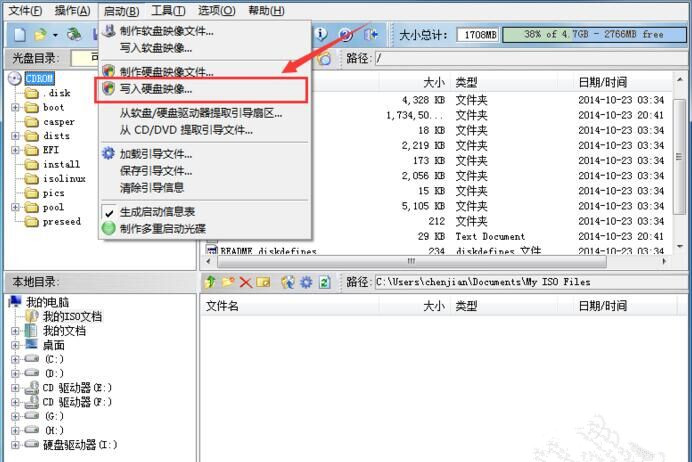
\includegraphics[width=0.5\textwidth]{tu1.jpeg}
\caption{图1}
\end{figure}

1.首先徐志伟老师说了一下目前中国的计算机开发者所处的状态。从一开始(包括徐老师)都只是建工程,再到在此基础上创新,他以微信为例,通过幽默的方式进行了解释。而对于当今的计算机社会,需要的不仅是我们的创新,更需要我们作为引领者,所以我们目前的状态就是步入引领。所谓引领者,徐老师举了个例子,当你做一件觉得正确的事,别人总会说三道四,你可以听一下他们的意见,但是你不一定的改正,因为你做的是引领者,你要引领他们沿着你的方向走。\\*

2.其次说了目前中科院计算所现在的项目\\*

(1)海运计算系统,它是中科院NICT先导专项,从2010到2017年春节结题\\*

(2)内存计算机体系结构,它是基金委的一个项目\\*

(3)软件定义的计算,这是科技部的一个项目\\*
\begin{figure}[!htb]
\centering
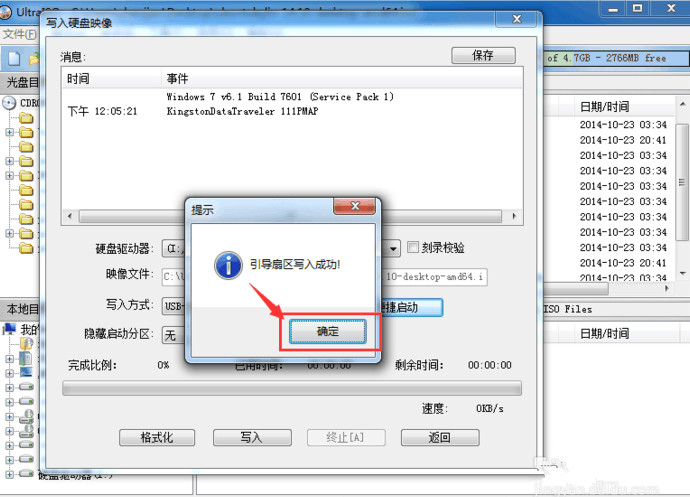
\includegraphics[width=0.5\textwidth]{tu3.jpeg}
\caption{图2}
\end{figure} 

3.徐老师说一下我们行业的基础性挑战:能效与速度增长的失配。通过一个折线图可以清楚的看到目前大数据的速度可以每焦耳达到十亿次(1TOPJ),而能效却已低到20-200KOPJ.这个问题是现在很大大挑战。\\
  
4.徐老师重点介绍了由58所的陈云霁和陈天石,领导研究出了寒武纪神经网络加速器。它将计算机的性能提高了1000倍,即从每焦耳十亿次到万亿次,这是一次很伟大的创举,同年两人都获得了“杰出青年”。\\
  
5.讲了一下“算礼”,所谓算礼就是用类似算法的语句,清晰,简洁的将计算机内部描述出来,这个词现在还么有明确的定义,所以徐老师自己起了一个名字,这也是他目前所要做的工作。\\
  
此次报告我能听懂的只有这些,有很多专业知识,我不太理解。但是,徐老师说的“一万小时”对我感触很深。所谓的一万个小时,就是你这一万个小时都在做一件事,是集中注意力去做的,哪怕只有五百小时,对于我们入门者来说也是很大的成功,他说这五百小时是你动手去做的时间,至于学习相关知识课本啊,都不抱括期内。我觉得他这个观点和郑老师“不谋而合”,我记得老师说过每天工作八小时,你要学习额外知识放在八小时之外。他说现在他们研究生生面试,看的不是分数,而是注重看你能力,不要求你门门精通,只要一门学的精通也是一种能力,这也是现在普遍高校的一个弊端。所以中科院现在不硬件要求研究生发表论文,博士生由原来的三篇减少到两篇,这虽然可以减少学生的毕业压力,可以更好的做研究,但是,也有不少学生因此放松精力,不在那么努力搞科研,所以这个问题在高校之中还是存在不少争议。\\
  
这是我来了之后听得第一个报告会,我觉得目前我很缺少动手锻炼、独立思考、语言表达、思维逻辑的能力,与老师说话永远说不上几句,而徐老师则是通过一种幽默的方式进行他的报告,就算我这个门外汉也觉得很想听听,所以我要学习的太多了,所以我要合理安排一下我这每天的八小时甚至更多,以次紧跟大家的步伐。
\end{document}



























